\documentclass[10pt,a4paper]{article}
\usepackage[T1]{fontenc}
\usepackage[brazil]{babel}
\usepackage[utf8]{inputenc}


\usepackage{ae,aecompl}
\usepackage{pslatex}
\usepackage{epsfig}
\usepackage{geometry}
\usepackage{url}
\usepackage{textcomp}
\usepackage{ae}
\usepackage{subfig}
\usepackage{indentfirst}
\usepackage{textcomp}
\usepackage{color}
\usepackage{setspace}
\usepackage{verbatim}
\usepackage{mathtools}
\usepackage{amsmath}


\linespread{1.5}
\geometry{ 
	a4paper,	% Formato do papel
	tmargin=30mm,	% Margem superior
	bmargin=40mm,	% Margem inferior
	lmargin=20mm,	% Margem esquerda
	rmargin=20mm,	% Margem direita
	footskip=20mm	% Espaço entre o rodapé e o fim do texto
}
\include{abaco} 
\renewcommand{\thetable}{\Roman{table}}
\newcommand{\x} {$\bullet$}


\begin{document}
% CAPA
\begin{titlepage}
\thispagestyle{empty}
  \begin{center} {\large \textbf{UNIVERSIDADE~ESTADUAL~DE~CAMPINAS}} \end{center}
  \begin{center} {\large INSTITUTO~DE~COMPUTAÇÃO}                    \end{center}
  \vspace{0.1cm}
  \begin{center}
  \begin{minipage}[tl]{31mm}
    \ABACO{1}{9}{6}{9}{1}
  \end{minipage}
  \end{center}
  \vspace{0.3cm}
  \begin{center} 
    {\large \textsc{São totalmente válidas algumas das considerações sobre a
Correlação de Pearson presentes na literatura?  }} 
    \\\vspace{0.5cm}
    {\textsl{Relatório do primeiro laboratório de MC920}}
    \\\vspace{1cm}
    \begin{tabular}{rl}
	  \textbf{Aluno}:   Carlos~Eduardo~Machado &  
	  \textbf{RA}:          059582 \\ 
	  \textbf{Aluno}:        Tiago~Chedraoui~Silva & 
	  \textbf{RA}:        082941 \\
	  \textbf{Aluno}:        William~Marques~Dias & 
	  \textbf{RA}:        065106 \\
	\end{tabular}
  \end{center}
  \vspace{0.5cm}

  \begin{abstract}
O coeficiente de correlação de Pearson é amplamente usado para
comparar imagens, contudo ele apresenta sérias limitações. Esse
trabalho consistiu na validação da análise realizada no Artigo ''The
Ineffectiveness of the Correlation Coefficient for Image Comparisons''.
  \end{abstract}
  % Sumário
  \tableofcontents
\end{titlepage} 

\vspace{2mm}
\newpage

\section{Introdução}
O coeficiente de correlação de Pearson é amplamente amplamente
utilizado na análise estatística, reconhecimento de padrões e
processamento de imagens.
Na área de processamento de imagens ele é utilizado na comparação de
duas imagens para fins de registro de imagens, reconhecimento de
objetos, e medição disparidade. Para imagens digitais monocromáticas, a correlação de Pearson é definido como :

\begin{equation}r = \frac{  
\displaystyle{\sum_{i} (x_i-\bar{x})(y_i-  
\bar{y})}}{\displaystyle{\left[  
\sum_{i}(x_i-\bar{x})^2  
\sum_{i}(y_i-\bar{y})^2\right]^{1/2}}}  \label{eq:r}
\end{equation}  

Onde $x_i$ é a intensidade dos pixels na imagem 1, $y_i$ é a
intensidade dos pixels na imagem 2,$\bar{x}$ é a intensidade média da
imagem 1 e $\bar{y}$ é a intensidade média da imagem 2.

O coeficiente tem valor $r=1$ se as duas imagens são absolutamente
idênticas, $r=0$ se são totalmente não correlacionadas e $r=-1$ se elas
são totalmente anti-correlacionadas, por exemplo se uma imagem é o
negativo da outra.

O coeficiente de Pearson pode ser utilizado em
aplicações de segurança, como, por exemplo, vigilância. Normalmente, 
o coeficiente de relação é usado para comparar duas imagens do mesmo
objeto ou cena durante vários momentos diferentes.

Não obstante à sua utilização, o coeficiente de correlação possui
diversas limitação, sendo considerado ineficaz em alguns papers.% ~\cite{paper}.
 
Assim, o objetivo deste trabalho é apresentar, através de exemplos, o
desempenho do coeficiente para comparações de imagens, especialmente
em aplicações de segurança e, posteriomrente, compará-las às considerações existentes na literatura.

%O paper é organizado a seção conclui

\section{Métodos}

Desenvolveu-se em python um programa de análise de imagens baseada no
coeficiente de correlação de pearson. 
Dado duas imagens para analisar duas imagens, sendo a imagem original dada por $x$  e a
imagem modificada por $y$ na equação \eqref{eq:r}, retorna-se o valor de $r$.

Inicialmente, para a análise do coeficiente, utilizou-se algumas imagens
previamente analisadas no artigo ´´The Ineffectiveness of the Correlation
Coefficient for Image Comparisons'' através do qual pretendíamos
confirmar os resultados obtidos.

Posteriormente, procurou-se alterar outra imagem com a
sobreposição de outra imagem. Alterou-se algumas características da
imagem sobreposta, como por exemplo, a posição, a opacidade, para
analisar os efeitos no cálculo do coeficiente produzidos por tais modificações. 

% \subsection{Código}

\newpage
\section{Resultados}

Utilizando as figuras \ref{fig1} e \ref{fig1Diff}usados no artigo ´´The Ineffectiveness of the Correlation
Coefficient for Image Comparisons'', na qual há uma simples
sobreposição de uma palavra sobre a imagem, obtemos um valor de r de
aproximadamente 0.89, enquanto no artigo o valor de r obtido vale 0.94.

\begin{figure}[h!]
\begin{center}
\subfloat[Imagem original]{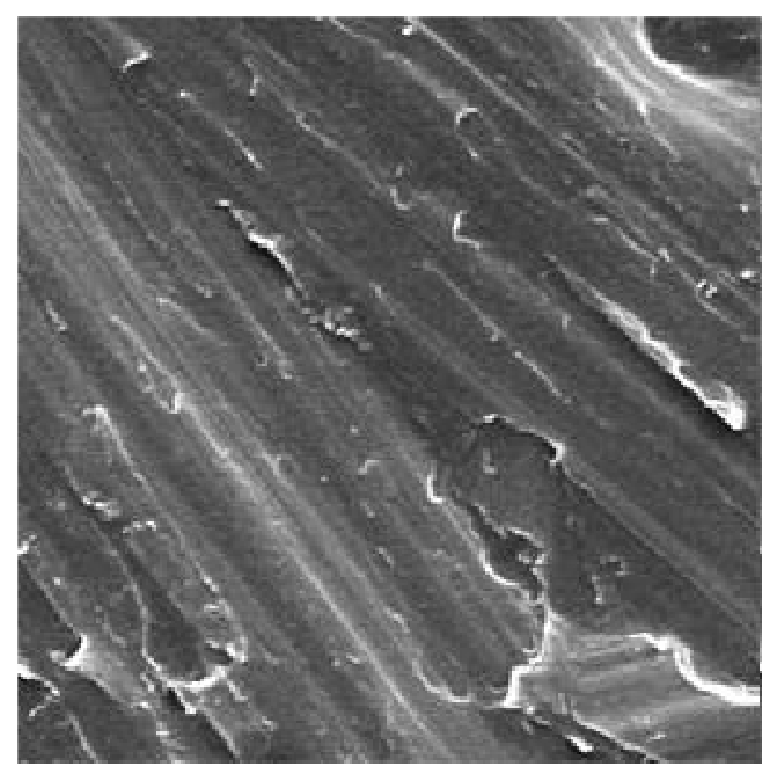
\includegraphics[scale=0.45]{photos/c1a}\label{fig1}}
\hspace{10mm}
\subfloat[Sobreposição de uma palavra sobre a imagem]{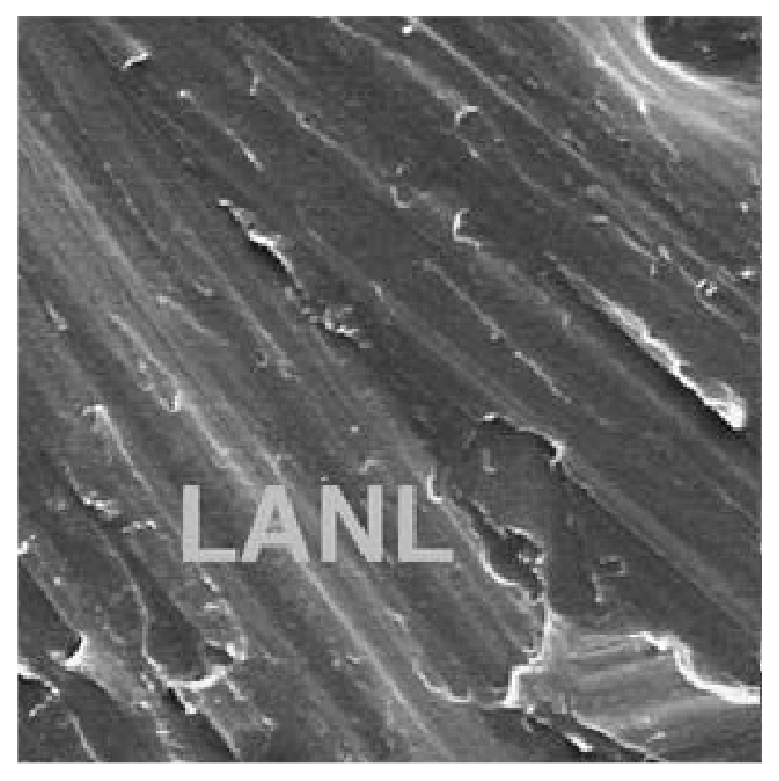
\includegraphics[scale=0.45]{photos/c1b}\label{fig1Diff}}
\caption{Comparação entre uma imagem original e outra com sobreposição
  de palavra}
\end{center}
\end{figure}

Para as imagens \ref{fig2} e \ref{fig2Diff}, na qual retira-se um
clips da imagem original, obteu-se um valor de r=0.90
enquanto no artigo r=0.98.
%figura clips

\begin{figure}[h!]
\begin{center}
\subfloat[Original]{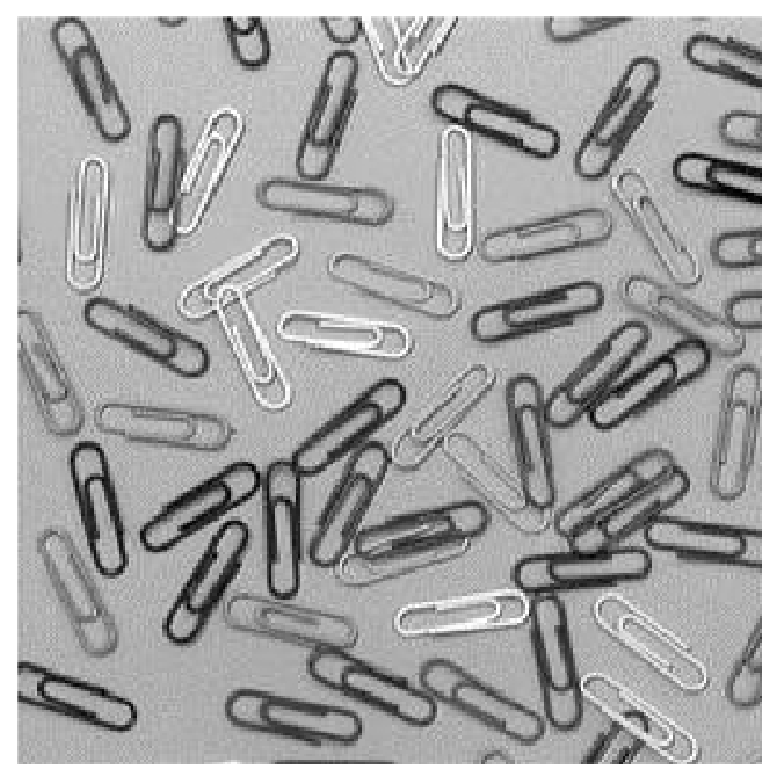
\includegraphics[scale=0.45]{photos/c2a}\label{fig2}}
\hspace{10mm}
\subfloat[Remoção de um clips na imagem original]{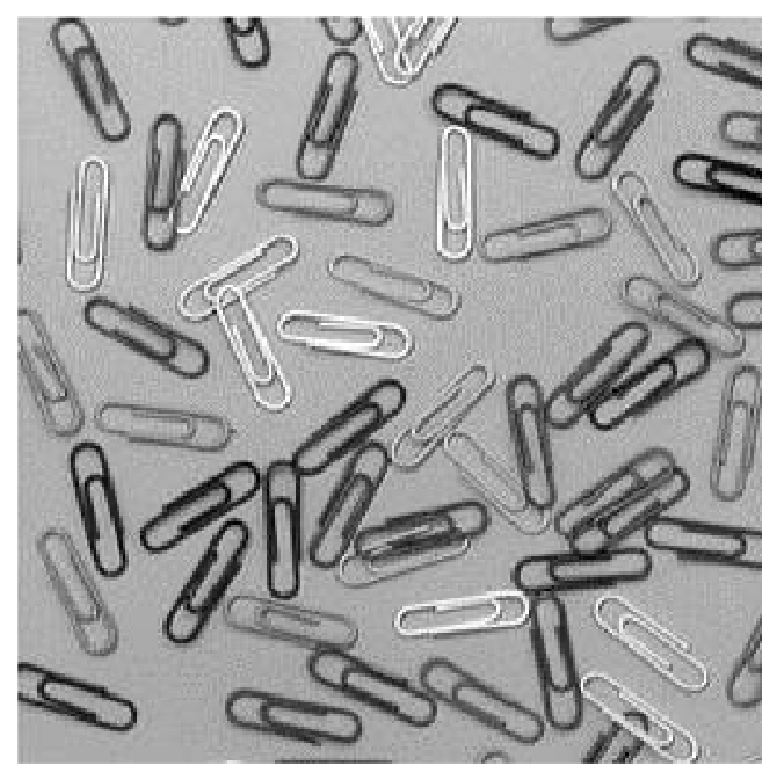
\includegraphics[scale=0.45]{photos/c2b}\label{fig2Diff}}
\caption{Comparação entre imagem com um objeto e outra sem esse objeto
 }
\end{center}
\end{figure}

\newpage

Para a imagem original \ref{fig3}, houve uma sobreposição da palavra
''CWT'' na imagem \ref{fig3Diff1} e na imagem \ref{fig3Diff2},
porém em posição diferente. Obteve-se para a imagem \ref{fig3Diff1}
um valor de r=0.99 se comparado à original e para a imagem \ref{fig3Diff2} 
um valor de r=0.98.
%m15 fig1
\begin{figure}[h!]
\begin{center}
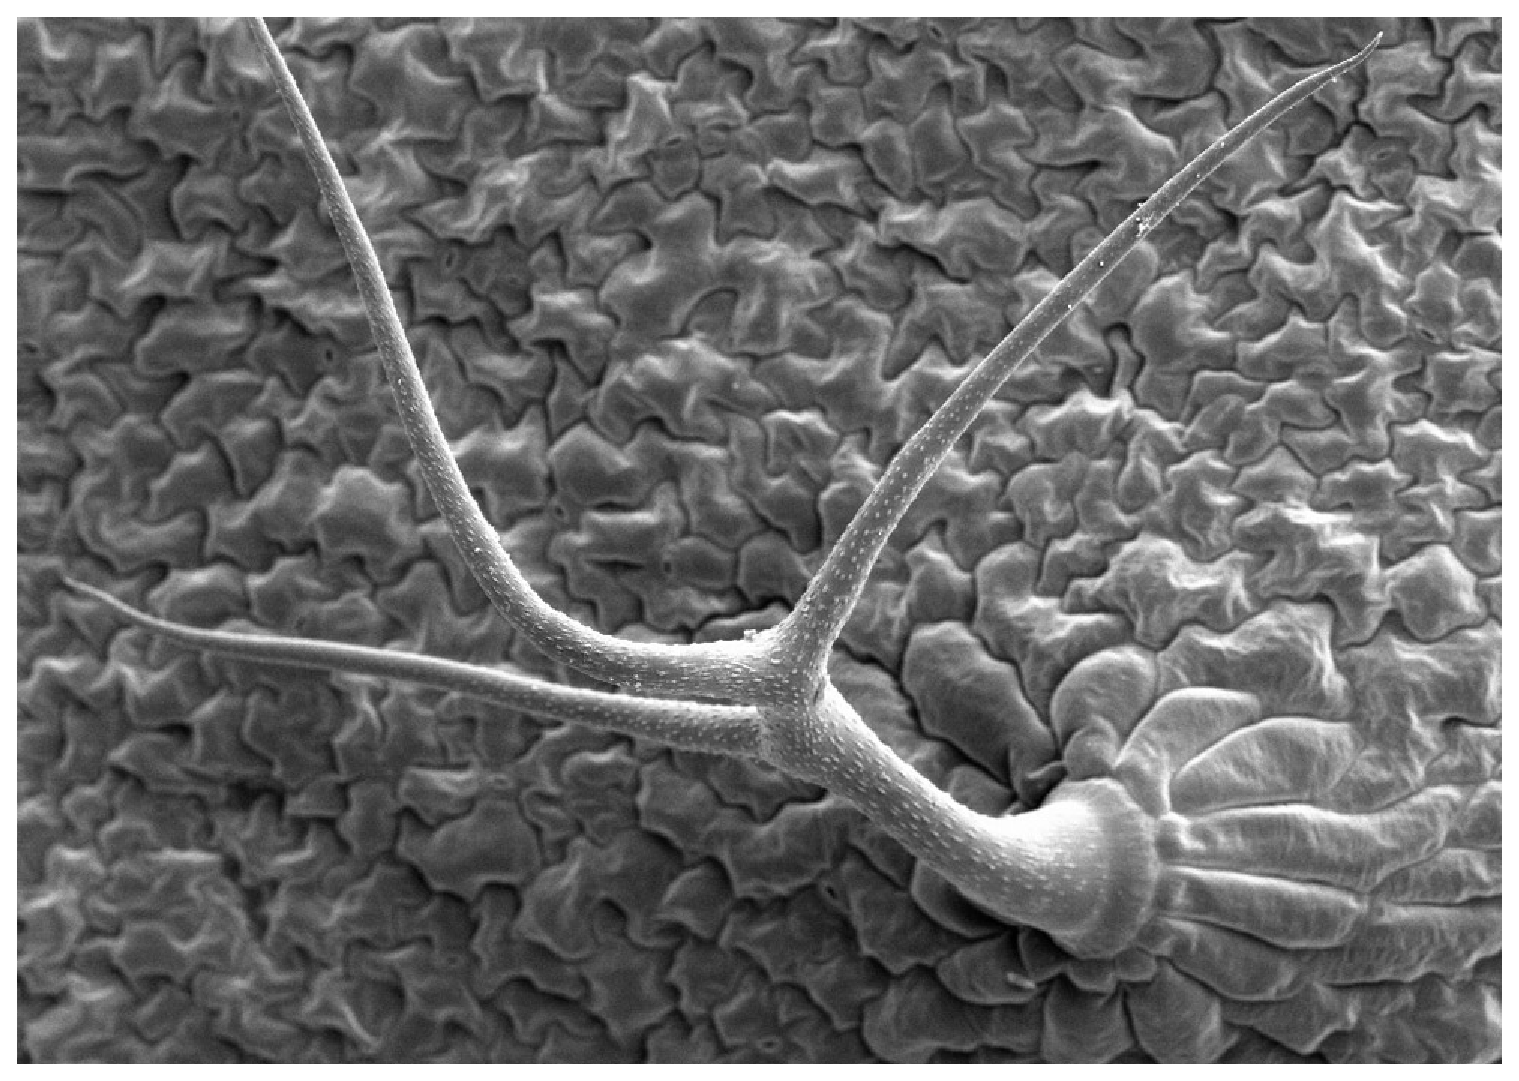
\includegraphics[scale=0.35]{photos/m15_tricome}\label{fig3}
\caption{Figura original a ser comparada}
\end{center}
\end{figure}



%m15 fig1
\begin{figure}[h!]
\begin{center}
\subfloat[Sobreposição da palavra CTW na figura original ]{\includegraphics[scale=0.22]{photos/m15_tricome_b}\label{fig3Diff1}}
\hspace{5mm}
\subfloat[Alteração da posição da palavra CTW  ]{\includegraphics[scale=0.22]{photos/m15_tricome_c}\label{fig3Diff2}}
\caption{Comparação entre a foto original e duas fotos compostas pela
  sobreposição de uma palavra à imagem original}
\end{center}
\end{figure}

\newpage


Para a imagem original \ref{fig3}, a imagem de Lena foi sobreposta nas
imagens \ref{fig3Diff3} e \ref{fig3Diff3}, sendo a primeira mais
transparente.
Se comparado à imagem original as imagens \ref{fig3Diff3} e
\ref{fig3Diff3} apresentam, respectivamente , r=0.93 e r=0.90 . 
%m15 fig1
\begin{figure}[h!]
\begin{center}
\subfloat[Sobreposição da foto de Lena com grau de transparência maior
 ]{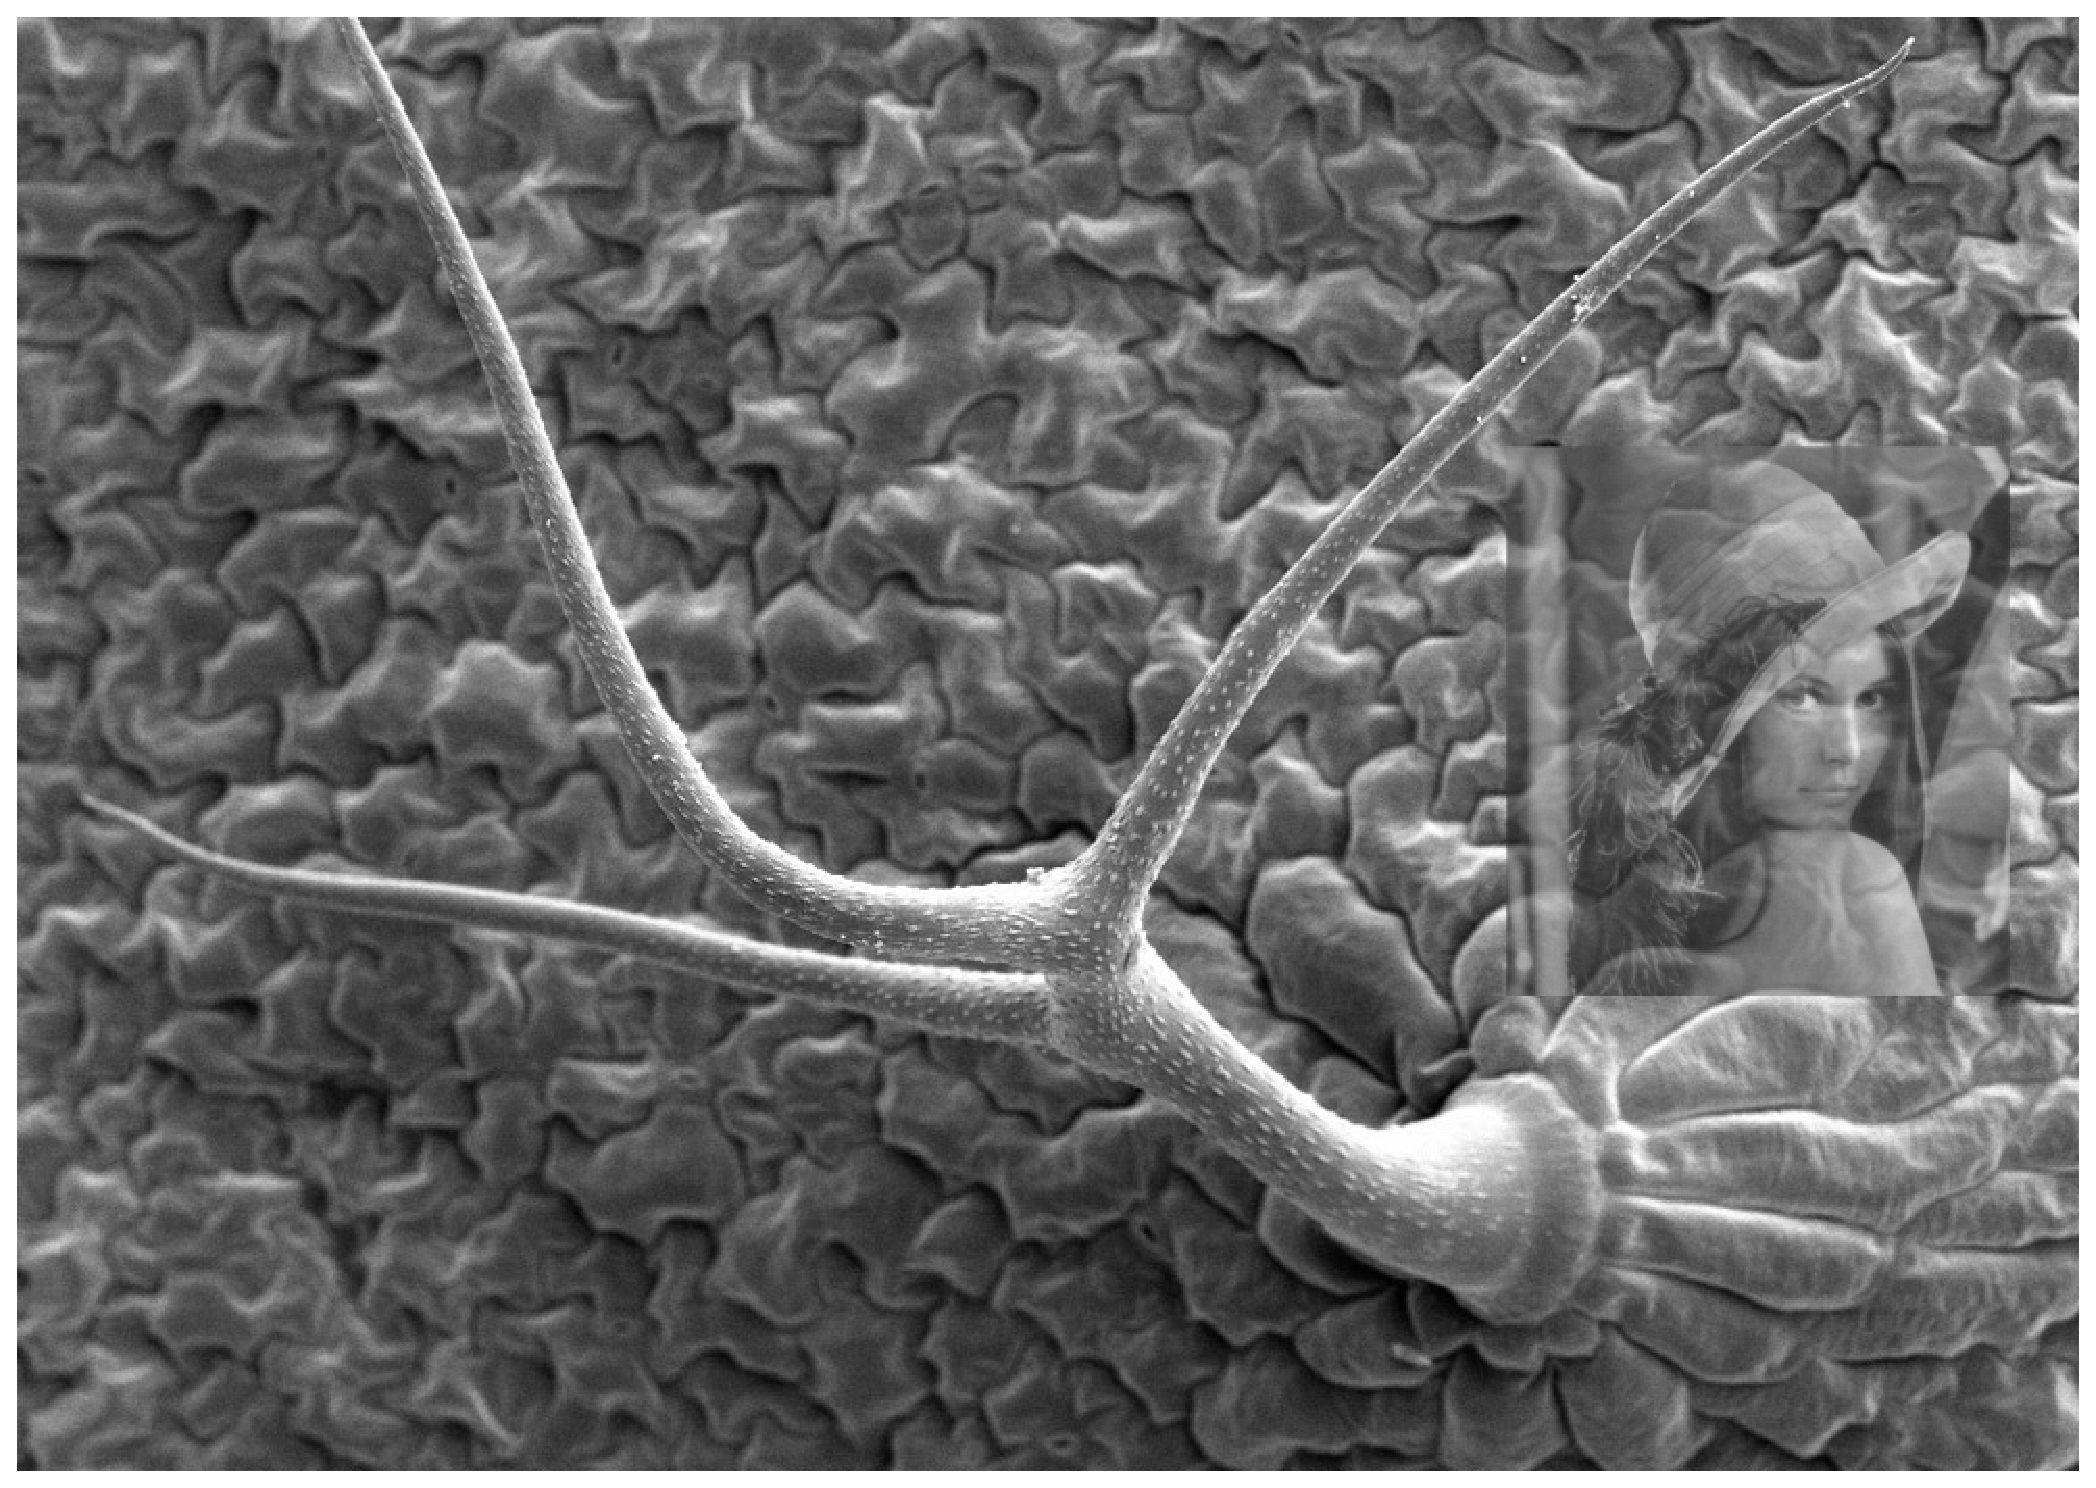
\includegraphics[scale=0.22]{photos/m15_tricome_d}\label{fig3Diff3}}
\hspace{10mm}
\subfloat[Sobreposição  da foto de Lena com grau de transparência
menor ]{\includegraphics[scale=0.22]{photos/m15_tricome_e}\label{fig3Diff4}}
\caption{Comparação entre a imagem original e duas imagens compostas pela sobreposição
  de uma outra imagem à imagem original}
\end{center}
\end{figure}

%livros remocao de objeto

Para a análise da remoção de um objeto da imagem, utilizou-se uma
sequência de imagens retiradas a cada 10s durante as quais é retirada
um livro de um estante de livro.
A figura \ref{fig4Diff1} é muito semelhante à imagem original, nas
figuras posteriores fez-se o movimento para a retirada do livro da
imagem, que é concluída na imagem \ref{fig4Diff4}.
Os valores de r podem ser vistos na tabela \ref{tab:livro}.

\begin{figure}[h!]
\begin{center}
\includegraphics[scale=0.35]{photos/livros/gBase} \label{livro}
\caption{Remoção de item: figura original a ser comparada}
\end{center}
\end{figure}

\newpage

\begin{figure}[h!]
\begin{center}
\subfloat[Imagem em t=0s ]{\includegraphics[scale=0.22]{photos/livros/g000}\label{fig4Diff1}}
\hspace{10mm}
\subfloat[Imagem em t=10s ]{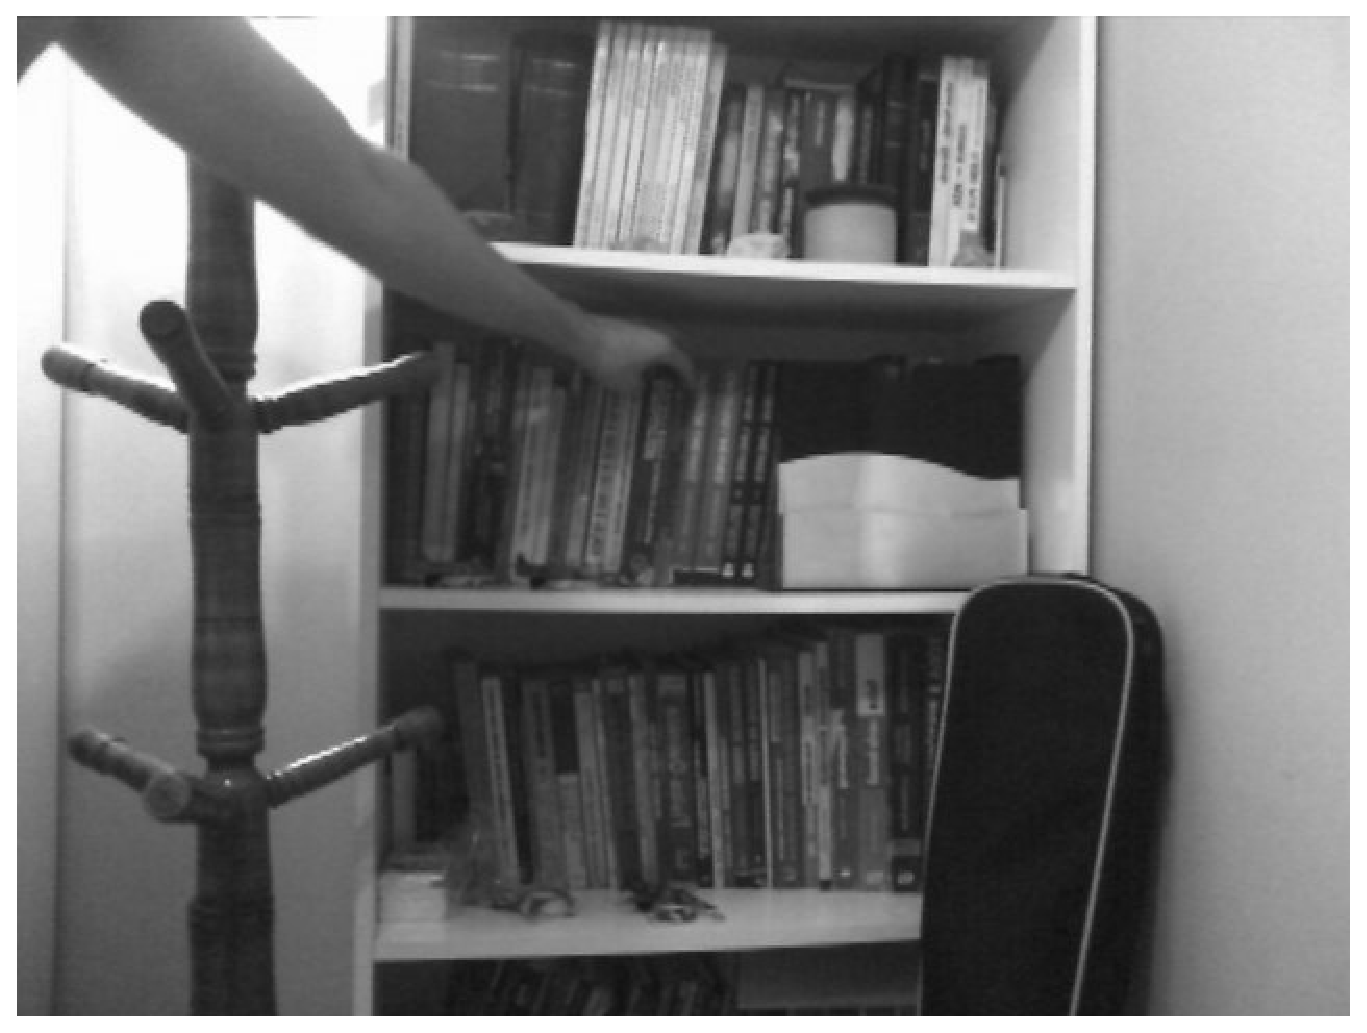
\includegraphics[scale=0.22]{photos/livros/g010}\label{fig4Diff2}}
\caption{Comparação entre a imagem original: tempo até 10 segundos }
\end{center}
\end{figure}


\begin{figure}[h!]
\begin{center}
\subfloat[Imagem em t=20s
 ]{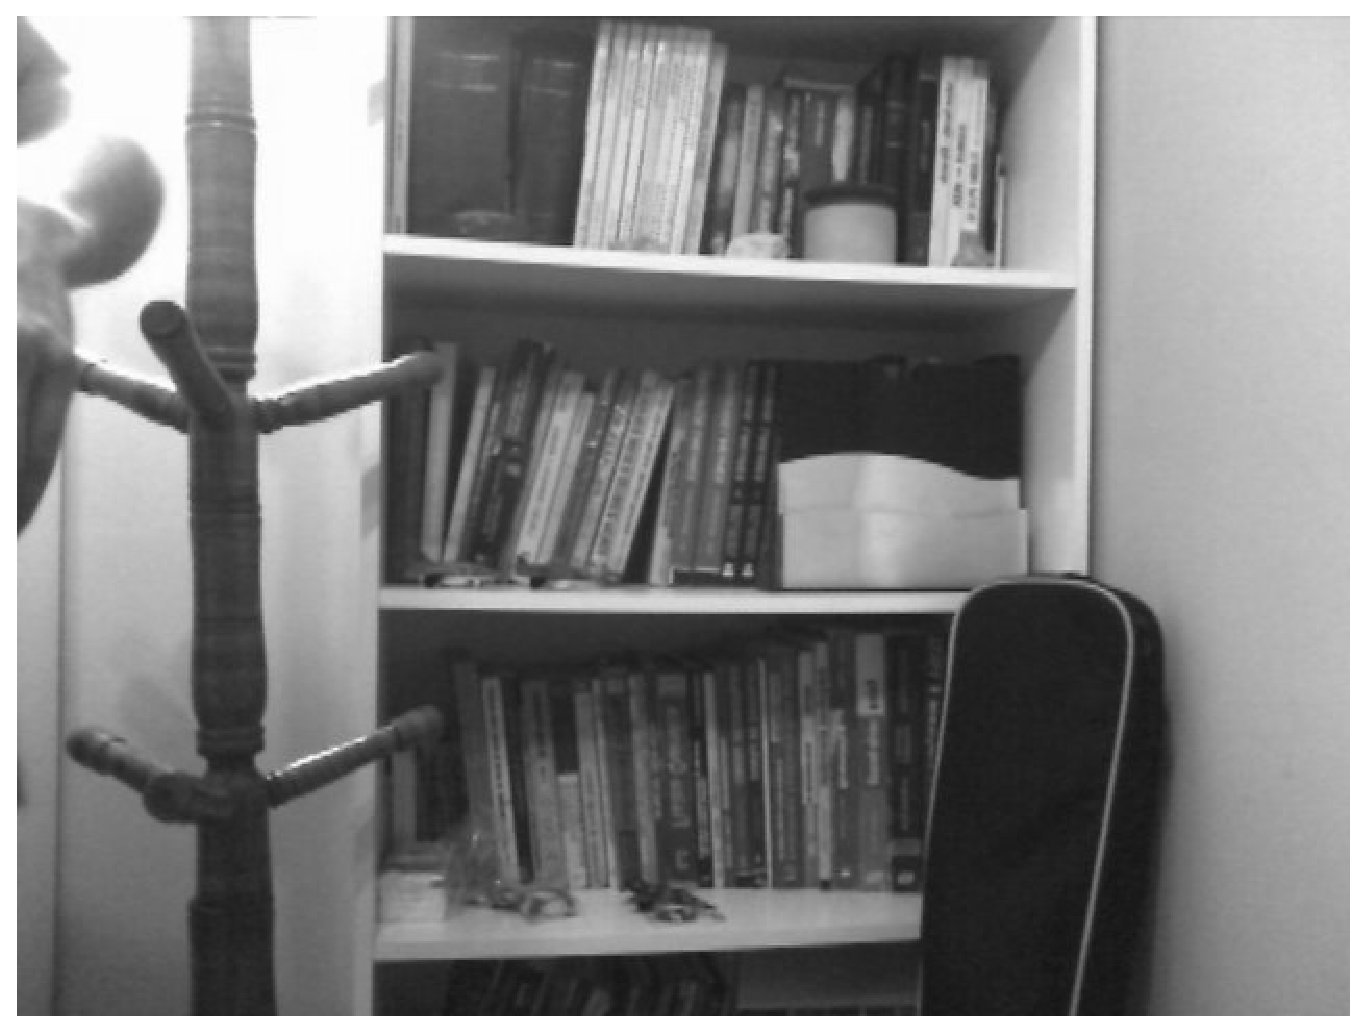
\includegraphics[scale=0.22]{photos/livros/g020}\label{fig4Diff3}}
\hspace{10mm}
\subfloat[Livro retirado: t=30s ]{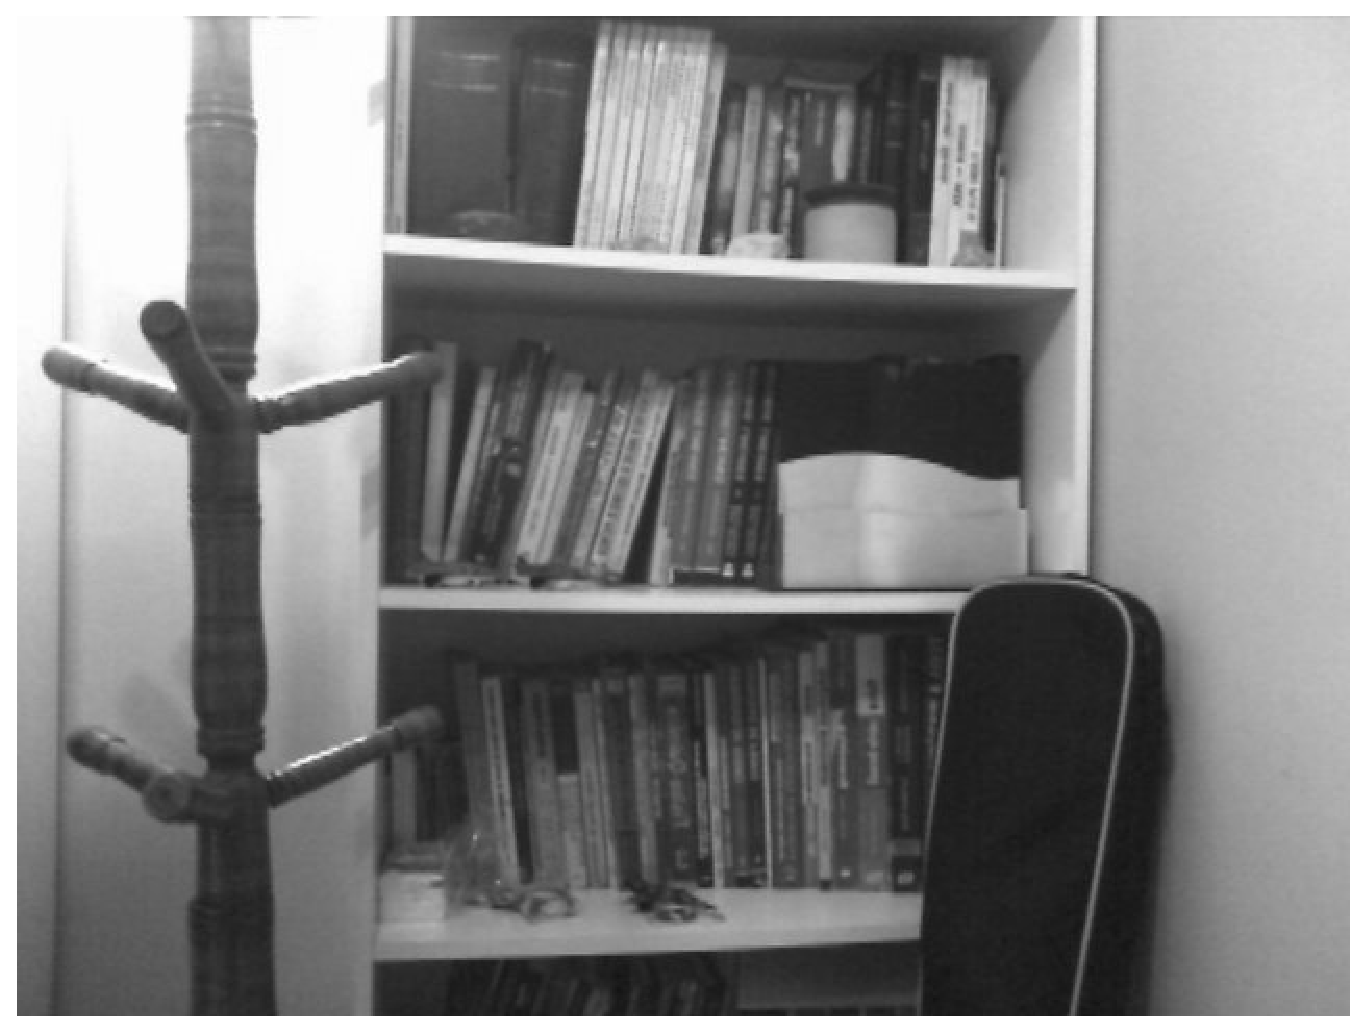
\includegraphics[scale=0.22]{photos/livros/g030}\label{fig4Diff4}}
\caption{Comparação entre a imagem original: tempo até 30s }
\end{center}
\end{figure}

%-%-%-%-%-%-%
% Tabela com 
% todos os 
% resultados
%-%-%-%-%-%-%
\begin{table}[h!]
  \begin{center}
    \caption{Valor do coeficiente de pearson para as várias imagens de
      remoção de um livro da estante}
    \begin{tabular}{|c|c|c|}
      \hline
      Figura original & Figura modificada & r\\
      \hline
      6 &  \ref{fig4Diff1} & 0.999600\\
      6 &  \ref{fig4Diff2} &  0.917454\\
      6 &  \ref{fig4Diff3} &   0.952869\\
      6 &  \ref{fig4Diff4} &   0.983264\\
      \hline
    \end{tabular}\label{tab:livro}
  \end{center}
\end{table}


%-%-%-%-%-%-%
% Teste Porta
%-%-%-%-%-%-%
\newpage
Para um outro teste dinâmico, obteve-se as sequências de imagens da
abertura de uma porta.

\begin{figure}[h!]
\begin{center}
\includegraphics[scale=0.35]{photos/porta/gBase} \label{porta}
\caption{Remoção de item: figura original a ser comparada}
\end{center}
\end{figure}

\begin{figure}[h!]
\begin{center}
\subfloat[Imagem em t=0s ]{\includegraphics[scale=0.22]{photos/porta/g000}\label{fig5Diff1}}
\hspace{10mm}
\subfloat[Imagem em t=10s ]{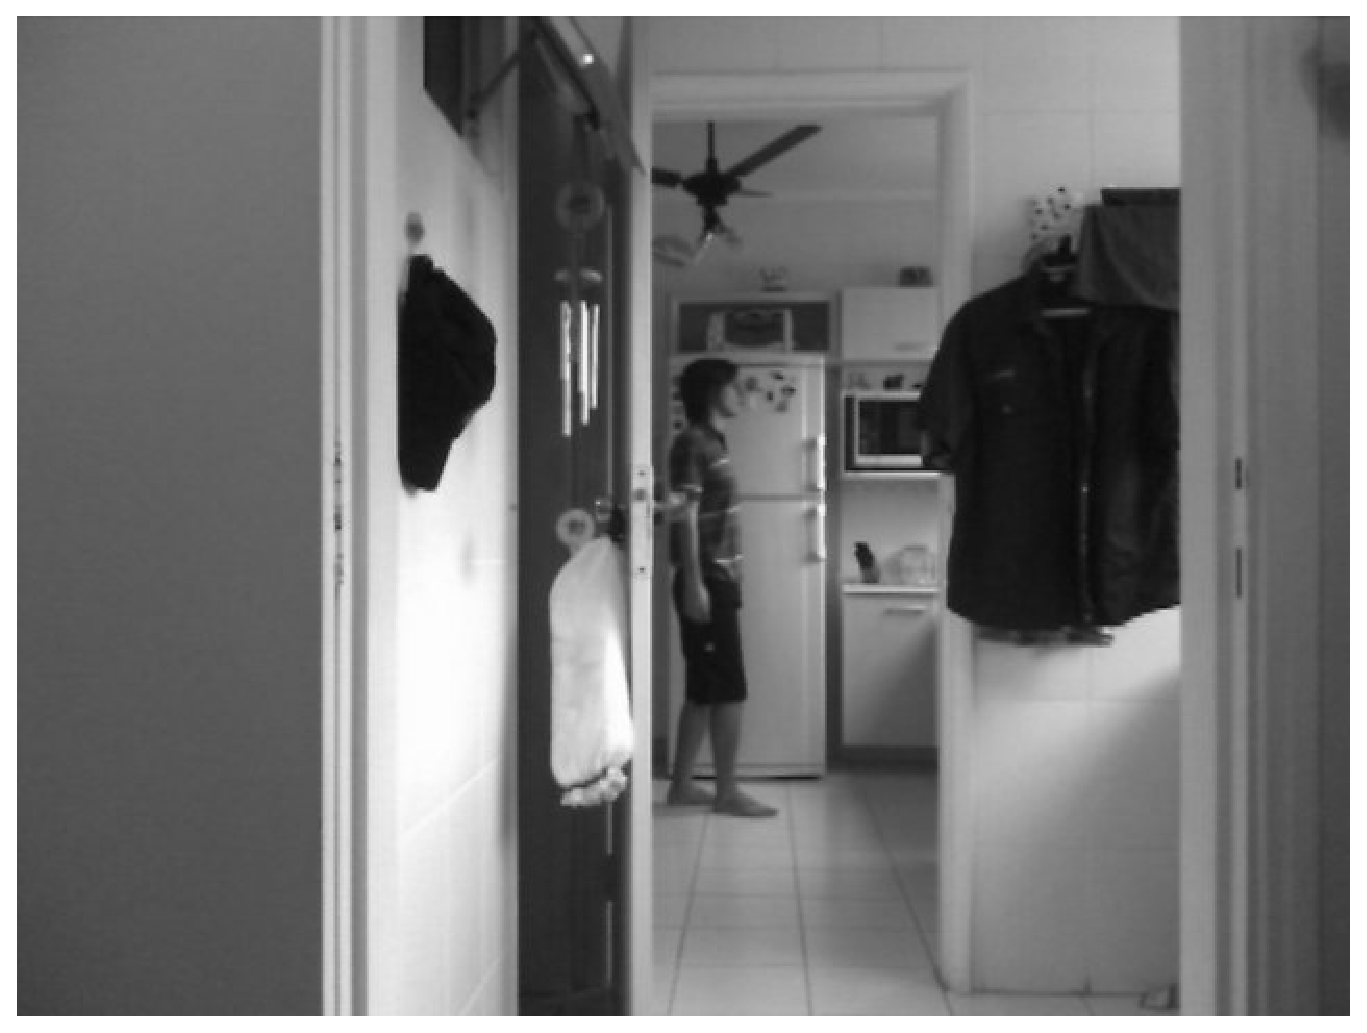
\includegraphics[scale=0.22]{photos/porta/g010}\label{fig5Diff2}}
\caption{Comparação entre a imagem original: tempos 0s e 10 s }
\end{center}
\end{figure}


\begin{figure}[h!]
\begin{center}
\subfloat[Imagem em t=20s
 ]{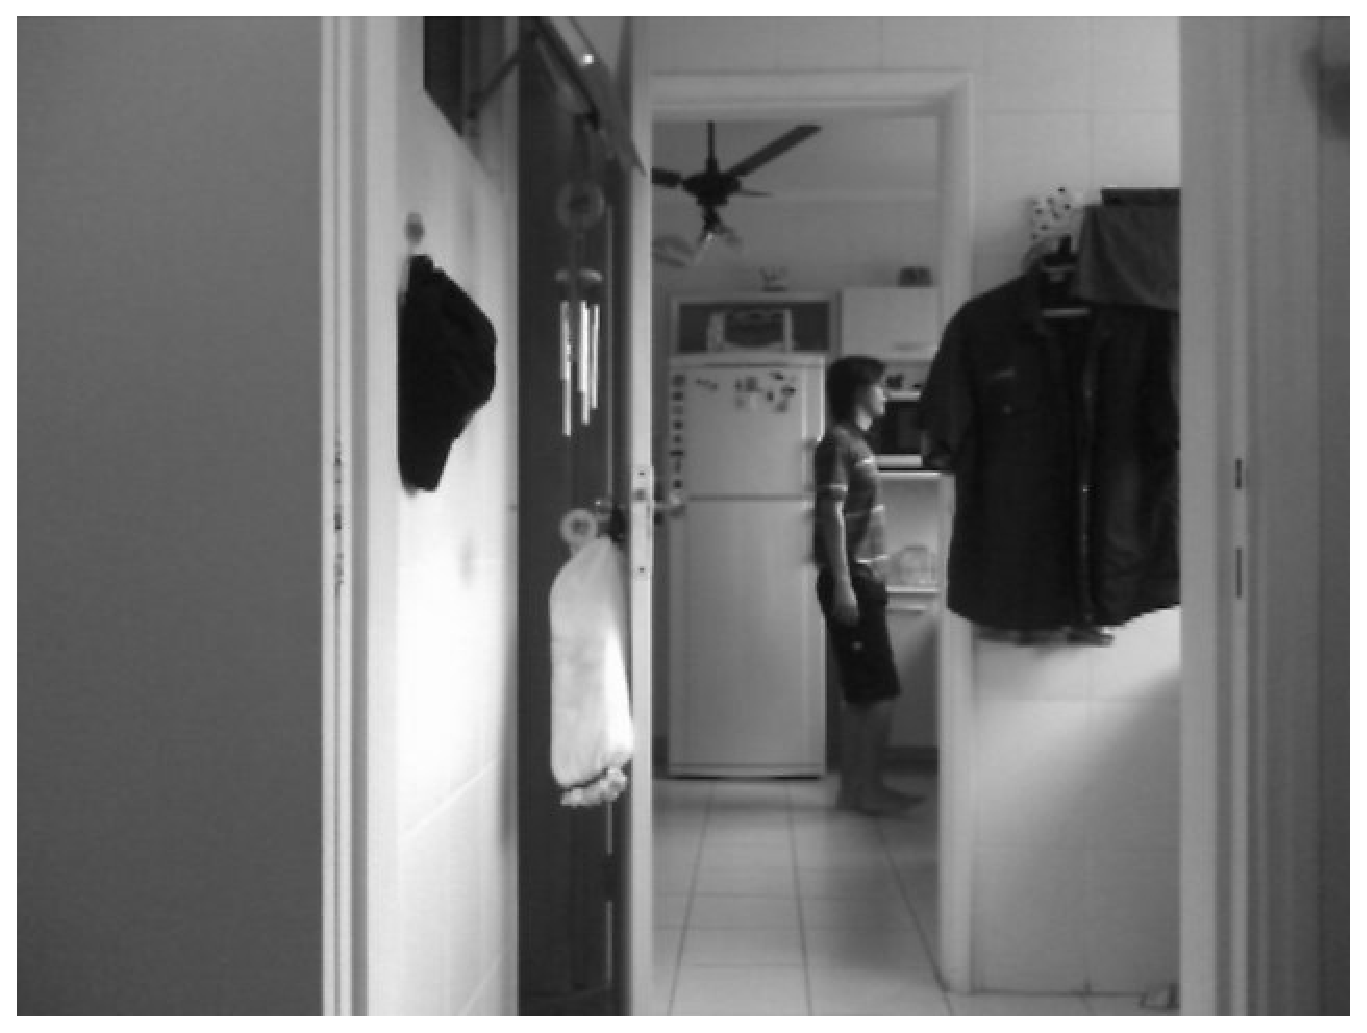
\includegraphics[scale=0.22]{photos/porta/g020}\label{fig5Diff3}}
\hspace{10mm}
\subfloat[Livro retirado: t=30s ]{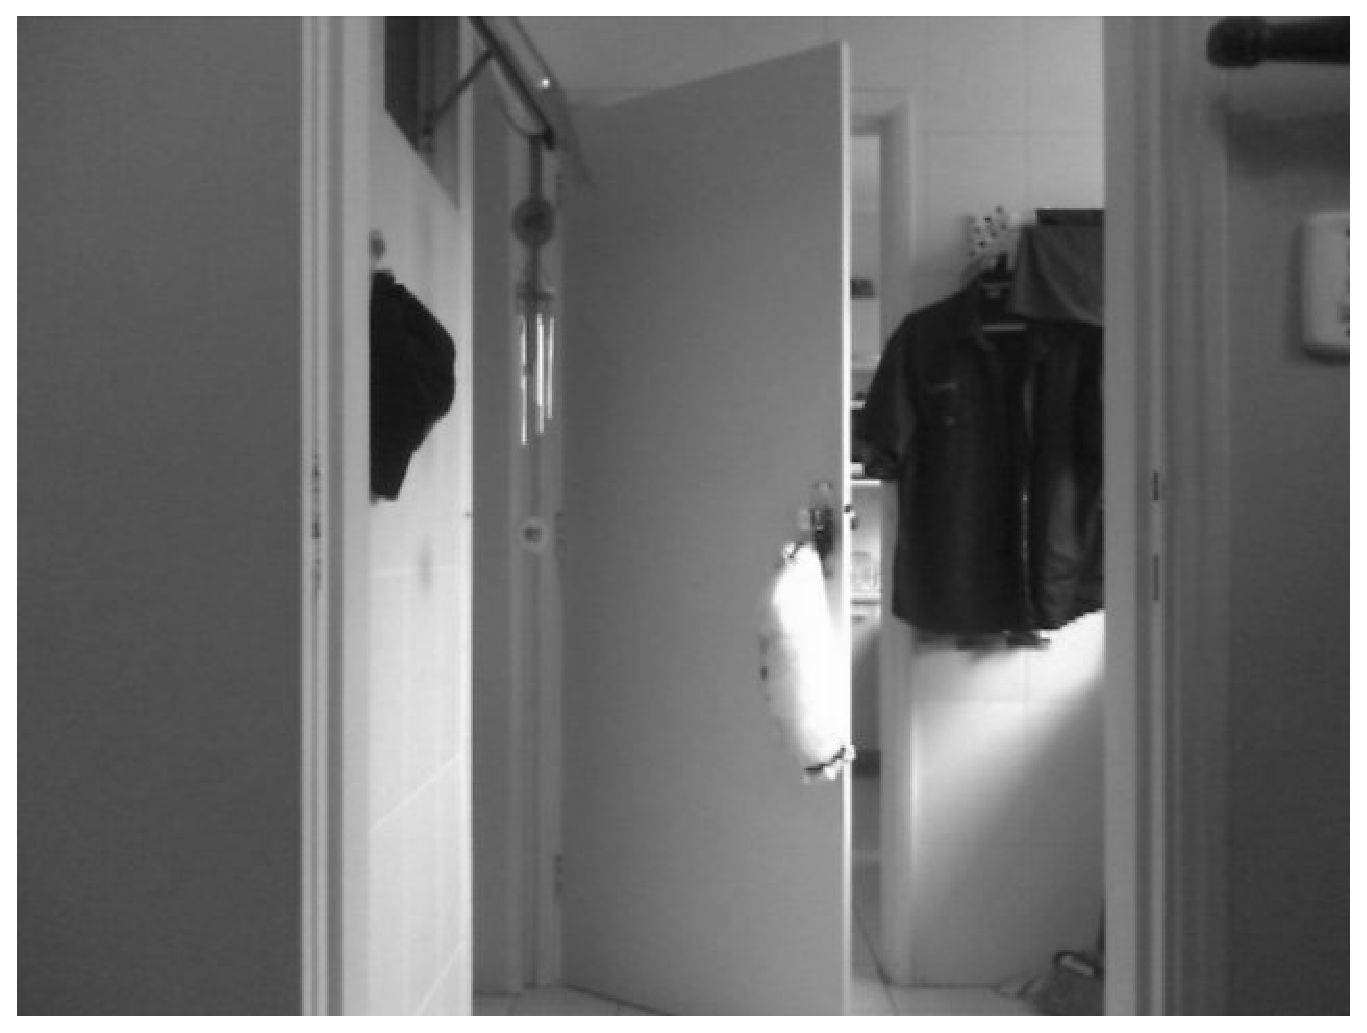
\includegraphics[scale=0.22]{photos/porta/g030}\label{fig5Diff4}}
\caption{Comparação entre a imagem original: tempos 20s e 30s }
\end{center}
\end{figure}


\begin{figure}[h!]
\begin{center}
\subfloat[Imagem em t=40s
 ]{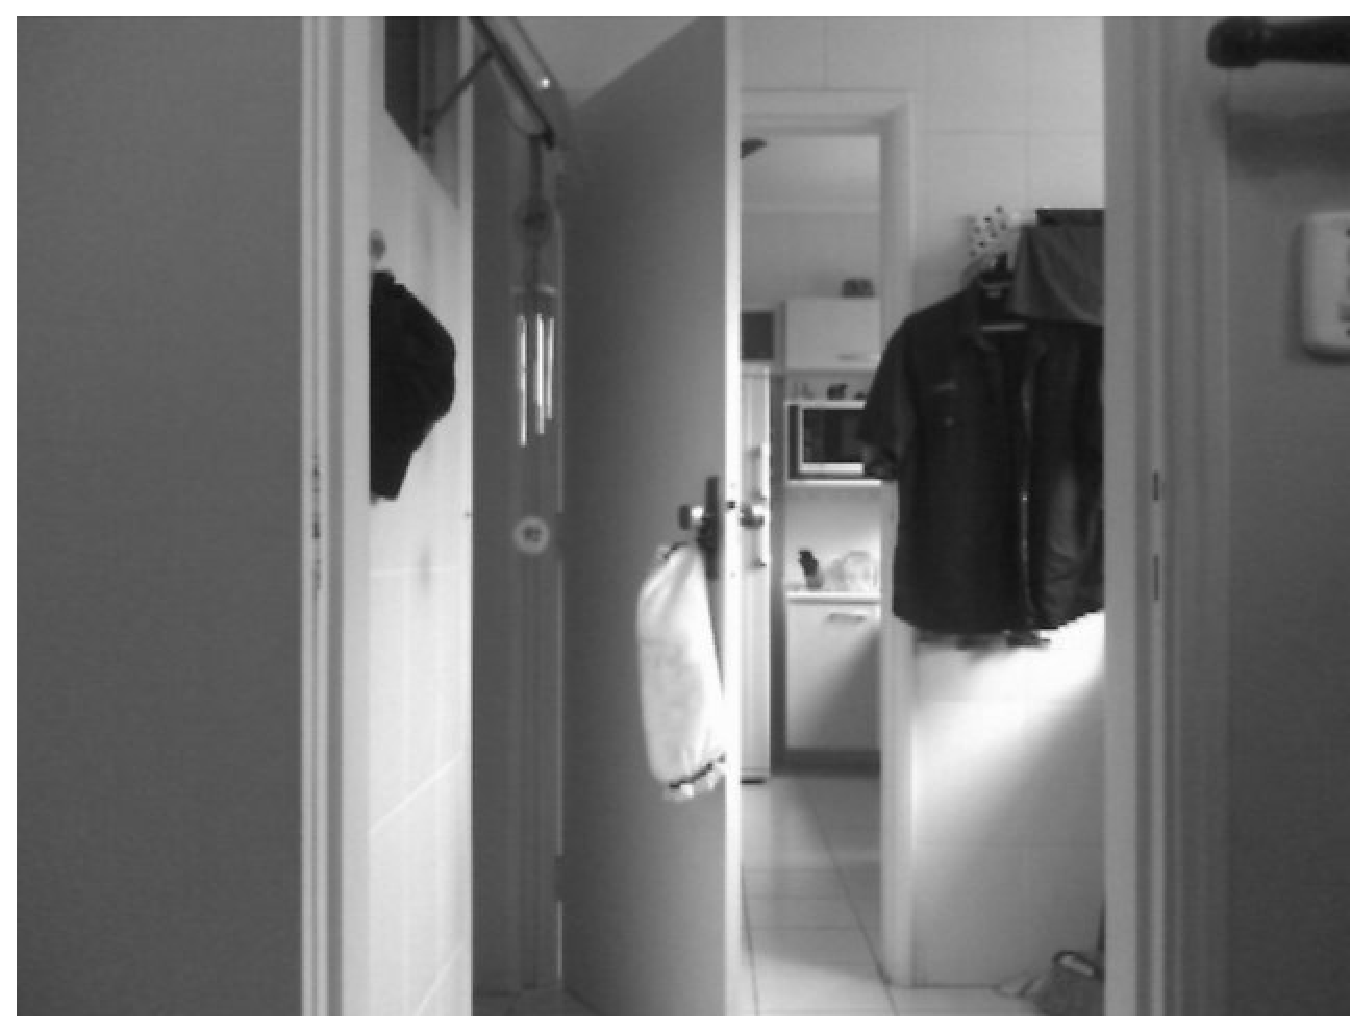
\includegraphics[scale=0.22]{photos/porta/g040}\label{fig5Diff5}}
\hspace{10mm}
\subfloat[Imagem em t=50s ]{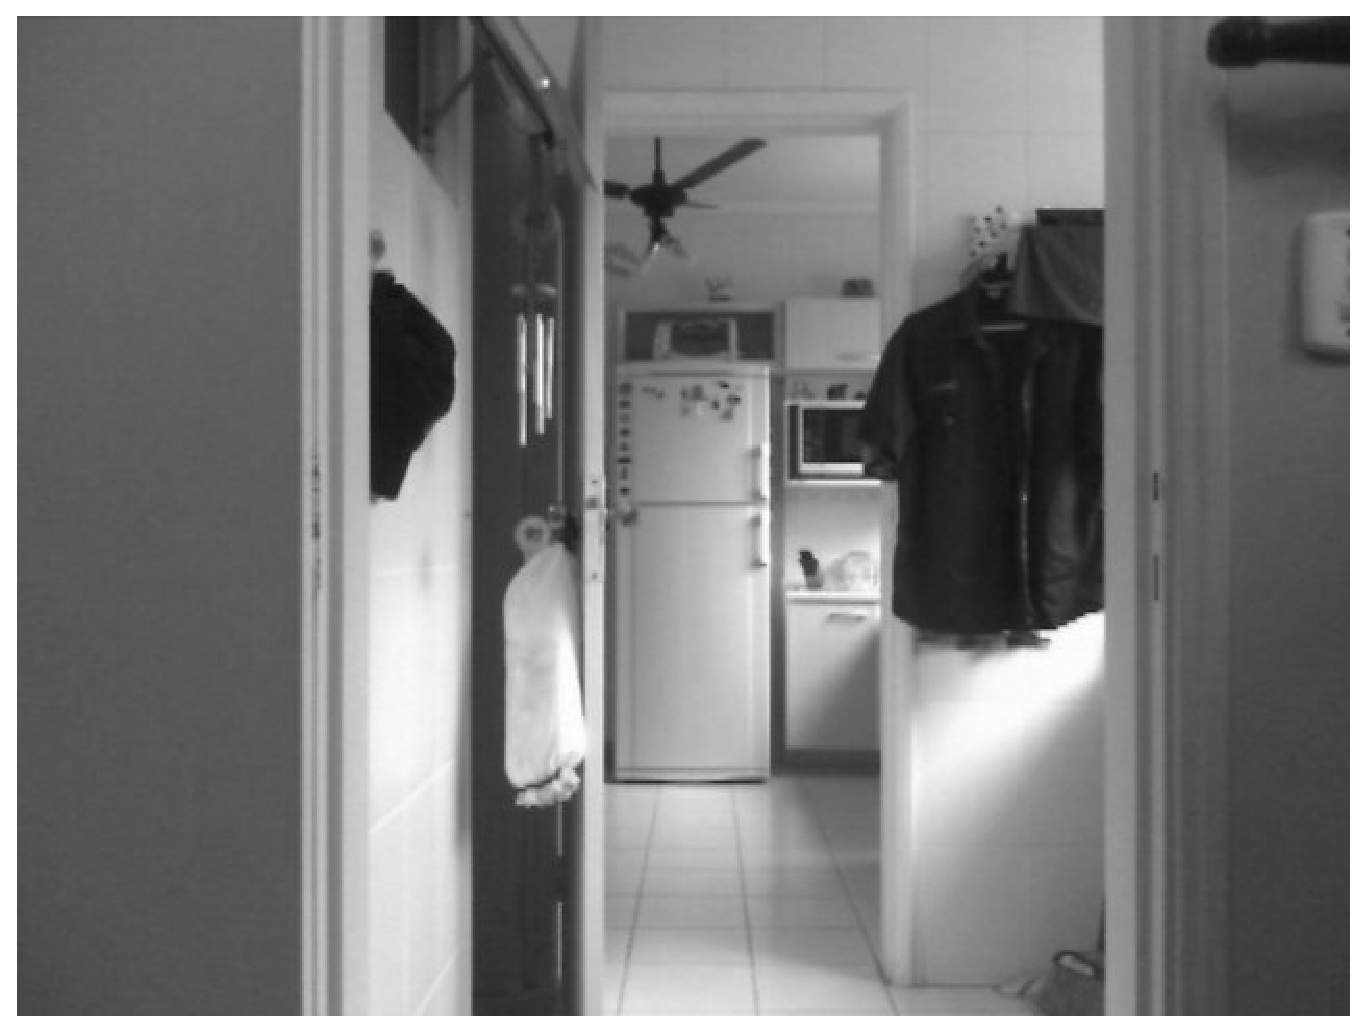
\includegraphics[scale=0.22]{photos/porta/g050}\label{fig5Diff6}}
\caption{Comparação entre a imagem original: tempos 40s e 50s }
\end{center}
\end{figure}

%-%-%-%-%-%-%
% Tabela com 
% todos os 
% resultados
%-%-%-%-%-%-%
\begin{table}[h!]
  \begin{center}
    \caption{Valor do coeficiente de pearson para sequência de imagens
      de abertura de um porta}
    \begin{tabular}{|c|c|c|}
      \hline
      Figura original & Figura modificada & r\\
      \hline
      10 &  \ref{fig5Diff1} & 0.996326\\
      10 &  \ref{fig5Diff2} & 0.995717\\
      10 &  \ref{fig5Diff3} & 0.952222\\
      10 &  \ref{fig5Diff4} & 0.862955\\
      10 &  \ref{fig5Diff5} & 0.798436\\
      10 &  \ref{fig5Diff6} & 0.818334\\
      \hline
    \end{tabular}
  \end{center}
\end{table}


\newpage
%-%-%-%-%-%-%
% Tabela com 
% todos os 
% resultados
%-%-%-%-%-%-%
\begin{table}[h!]
  \begin{center}
    \caption{Valor do coeficiente de pearson para todos as comparações}
    \begin{tabular}{|c|c|c|}
      \hline
      Figura original & Figura modificada & r\\
      \hline
      \ref{fig1} &  \ref{fig1Diff} &  0.887291 \\
      \ref{fig2} &  \ref{fig2Diff} &  0.907154\\
      \ref{fig3} &  \ref{fig3Diff1} & 0.994465\\
      \ref{fig3} & \ref{fig3Diff2} &  0.985331\\
      \ref{fig3} &  \ref{fig3Diff3} &  0.936883\\
      \ref{fig3} &  \ref{fig3Diff4} &  0.905874\\
      6 &  \ref{fig4Diff1} & 0.999600\\
      6 &  \ref{fig4Diff2} &  0.917454\\
      6 &  \ref{fig4Diff3} &   0.952869\\
      6 &  \ref{fig4Diff4} &   0.983264\\
      10 &  \ref{fig5Diff1} & 0.996326\\
      10 &  \ref{fig5Diff2} & 0.995717\\
      10 &  \ref{fig5Diff3} & 0.952222\\
      10 &  \ref{fig5Diff4} & 0.862955\\
      10 &  \ref{fig5Diff5} & 0.798436\\
      10 &  \ref{fig5Diff6} & 0.818334\\
      \hline
    \end{tabular}
  \end{center}
\end{table}


\section{Conclusão}
Utilizamos o coeficiente de correlação de Pearson  
 como método de comparação de imagens. Foram feitas diversas
 comparações de forma a obter-se uma gama de resultados suficientes
 para a análise do coeficiente.

O coeficiente de correlação de Pearson, assim como em outras
avaliações na literatura, demonstrou-se inefetivo. Portanto, os
resultados corroboram com o artigo de Eugene K. Yen e
Roger G. Johnston.

%Necessária?
%\section{Agradecimentos}

% ******************************************************
% 		REFERENCIAS BIBLIOGRÁFICAS
% ******************************************************
%\section{Referências}
\bibliographystyle{plain}
\begin{small}
  \bibliography{referencias}
\end{small}

\end{document}
